% !TeX root = ../main.tex
Supplementary material referenced from the main text.

\setcounter{figure}{0}
\setcounter{table}{0}
\renewcommand{\thefigure}{S\arabic{figure}}
\renewcommand{\thetable}{S\arabic{table}}
\renewcommand{\figurename}{Supplementary Figure}
\renewcommand{\tablename}{Supplementary Table}

\begin{table}[ht]
\centering
\caption{Operational definition of the problem BARCS addresses.  Referenced
from the Introduction.}
\label{tab:problem}
\small
\setlength{\tabcolsep}{5pt}
\begin{tabular}{p{0.22\textwidth}p{0.68\textwidth}}
\toprule
Component & Definition\\
\midrule
Observed data &
Guide counts $K_{gi}$, unfiltered full-library totals $N_i$, and a
prespecified sample design matrix $X$\\
Primary estimand &
A guide-level coefficient or contrast
$\mathbf{c}^\top\boldsymbol{\beta}_g$ conditional on the other columns of
$X$\\
Information unit &
An independent biological screen unit represented by a sequenced library;
additional reads refine that unit but do not create another one\\
Primary output &
Guide effect, standard error, $t$ statistic, residual degrees of freedom,
$p$-value, FDR, and dispersion diagnostics\\
Optional gene output &
An inverse-variance shared-effect Wald statistic with empirical-null
calibration; no Fisher or Stouffer step is required\\
Not identified &
Unobserved single-cell phenotypes, dependence among bins from one biological
pool, mechanistic growth dynamics, or uncertainty that would have required
missing biological replicates\\
\bottomrule
\end{tabular}
\end{table}

% !TeX root = ../../main.tex
\subsection{Finite-sample calibration is not guaranteed by the sampling model}
\label{sec:calibration}

The first analysis uses known truth rather than biological proxy labels.  We
simulated 200 genes with three guides per gene under the fitted beta-binomial
model, including 160 null genes, 27 independent libraries, a continuous dose,
and three batches.  The tested model therefore matches the data-generating mean
and variance families.  Gene probabilities use the prespecified directional
Stouffer summary for BARCS and the native gene statistic for MAGeCK-MLE.

\begin{table}[htbp]
\centering
\caption{Nominal-versus-realized error rates in the continuous-dose
beta-binomial simulation.  Type-I error is the fraction of 160 null genes with
$p<0.05$.  Empirical FDP is measured among calls at Benjamini--Hochberg FDR
0.05.  This single deterministic simulation is a diagnostic, not a claim of
uniform operating characteristics.}
\label{tab:type1}
\small
\setlength{\tabcolsep}{5pt}
\begin{tabular}{lrrrr}
\toprule
Method & Null type I & Power & Calls & Empirical FDP\\
\midrule
Naive binomial $z$ & 0.844 & 1.000 & 174 & 0.770\\
BARCS unmoderated $t$ & 0.081 & 1.000 & 46 & 0.130\\
BARCS moderated $t$ & 0.088 & 1.000 & 44 & 0.091\\
Official MAGeCK-MLE Wald & 0.038 & 0.975 & 41 & 0.049\\
\bottomrule
\end{tabular}
\end{table}

BARCS is anti-conservative in this example despite correct beta-binomial
simulation.  The guide-level null rate is 0.077, so the failure is already
present before gene aggregation.  No fitted guide reaches the lower
$\widehat\rho=0$ boundary; the truncation mechanism is therefore not the cause
in this simulation.  More generally, the model-based covariance treats
$\widehat\rho$ as fixed, and the residual-$t$ reference does not propagate
guide-specific dispersion uncertainty.  Moderation lowers the empirical FDP
but does not restore nominal type-I error.

Negative controls can diagnose this behavior, but evaluation must be separated
from estimation.  In the IL2RA FACS screen, 0.133 of 593 non-targeting guides
have raw $p<0.05$.  The tail-quantile calibration sets its scale from the
control tail, so measuring those same controls after calibration would be
circular.  Five-fold cross-fitting instead estimates each scale on four folds
and scores the omitted fold.  The resulting held-out rate is 0.049.  This is a
valid out-of-sample diagnostic of the scaling rule at the selected threshold;
it does not repair the correlation among bins from one donor or validate the
independent-library likelihood.

The processed Liang analysis provides a secondary, weaker diagnostic.  BARCS
has a macro-averaged null $p<0.05$ rate of 0.064.  Its reported calibration
error, 0.025, is the mean of the four cell-line-specific absolute errors, not
$|0.064-0.05|=0.014$.  MAGeCK-MLE has corresponding values 0.107 and 0.057.
Because the common matrix was normalized, ComBat-corrected, and rounded before
either fit, these values compare procedures on that transformed input but
cannot establish calibration of their count likelihoods.


\begin{figure}[htbp]
\centering
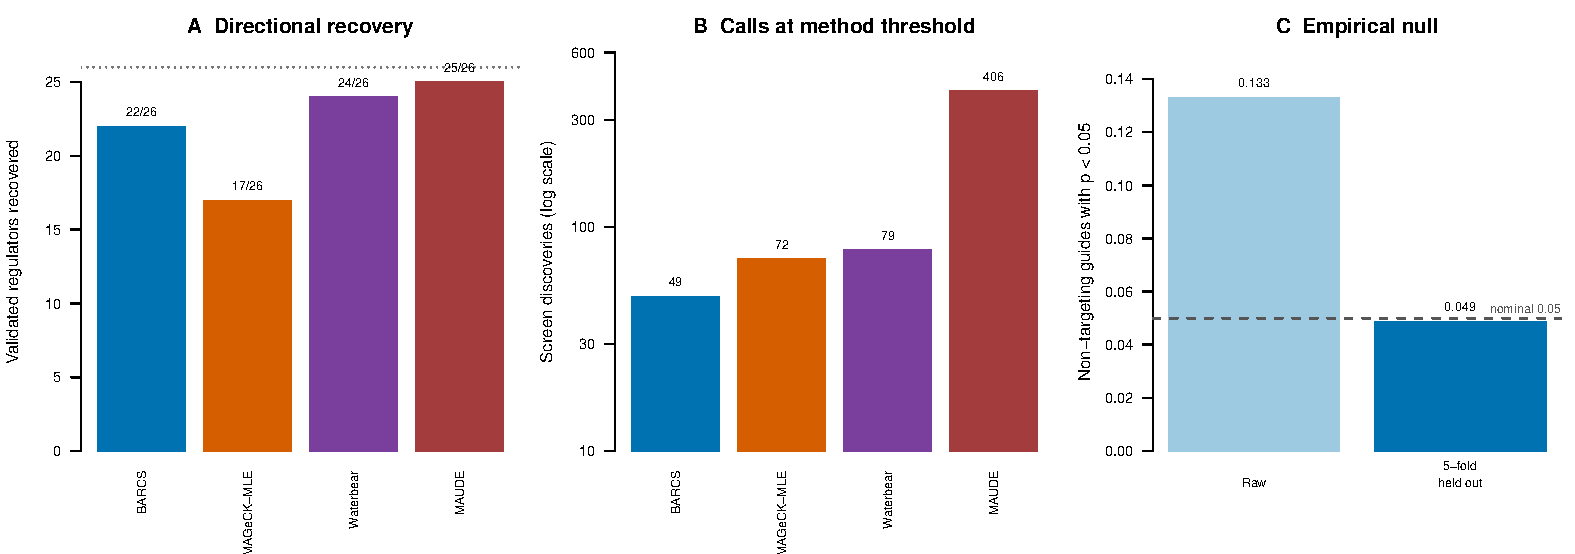
\includegraphics[width=\textwidth]{figures/waterbear_facs_main.pdf}
\caption{\textbf{Supporting ordered-bin IL2RA benchmark.}  (A) Directional
recovery of 26 independently validated regulators.  (B) Total discoveries at
each method's threshold (log scale).  (C) Empirical non-targeting-guide
$p<0.05$ rate before and after BARCS control calibration; the dashed line is
the nominal rate.}
\label{fig:waterbear}
\end{figure}

\input{sections/results/supp_ht29-cnv}

\paragraph{Additional multivariable and endpoint benchmarks.}
The following analyses test backward compatibility, multivariable effect
concordance, copy-number sensitivity, and preprocessing contracts.  They are
reported separately because none is a direct test of the primary longitudinal
generalization.

% !TeX root = ../../main.tex
\subsection{A multi-coefficient design on real data: GSE70038}

The benchmarks so far test one coefficient at a time.  GSE70038 is the case
where the design matrix earns its place: 64,747 guides in 16 libraries from two
glioblastoma stem-cell lines and two neural stem-cell lines, with duplicate
initial and terminal samples \citep{toledo2015pkmyt1}.  The scientific target is
four cell-line-specific terminal effects estimated \emph{jointly} against one
shared initial baseline.  Four separate two-group tests cannot express that: each
would re-estimate the baseline from its own pair, discarding the other twelve
libraries that inform it.  This is therefore not a continuous-phenotype
benchmark but the multivariable one, and it is the design MAGeCKFlute documents
as the canonical multi-condition layout.

We followed the design-matrix rules in Table~5 and Box~3 of the MAGeCKFlute
protocol \citep{wang2019mageckflute}.  The first column is one for every
library; each initial library has zeros elsewhere; and each terminal library
has one in exactly one of four cell-line columns.  The same $16\times5$ matrix
was supplied to beta-binomial regression and the official MAGeCK-MLE 0.5.9.5
executable.  MAGeCK used median normalization and its Wald inference.  For the
beta-binomial result, guide effects were summarized by their within-gene
median, and directional guide $p$-values were combined by Stouffer's method.
This aggregation is an explicit comparison device, not a proposed replacement
for MAGeCK's gene model.

The ``effect rank correlation'' reported below is calculated in this analysis,
not copied from GEO or the MAGeCKFlute paper.  Separately for each terminal
coefficient, we pair all genes available from both methods.  The
beta-binomial effect is the within-gene median guide coefficient, and the
MAGeCK effect is its official MLE beta.  We assign average ranks to these two
effect vectors and take their Pearson correlation, which is exactly Spearman's
rank correlation.  The 18,077 paired effects and their ranks for every
coefficient are included with the deposited analysis output.

\begin{table}[ht]
\centering
\caption{Effect concordance between \methodswatch{barcsblue} BARCS and
\methodswatch{mageckorange} official MAGeCK-MLE on GSE70038.  Jaccard is the
overlap divided by the union of the 200 most depleted genes from each method.
Higher agreement is better; column maxima are shown in bold.}
\label{tab:gse}
\begin{tabular}{lrr}
\toprule
Terminal coefficient & Spearman effect correlation & Top-200 Jaccard\\
\midrule
GSC0131 & \textbf{0.928} & 0.550\\
GSC0827 & 0.888 & 0.533\\
NSCCB660 & 0.905 & 0.544\\
NSCU5 & 0.915 & \textbf{0.562}\\
\bottomrule
\end{tabular}
\end{table}

Concordance here is the validation rather than the finding.  The comparison is
not circular: beta-binomial regression conditions on each library total, whereas
MAGeCK uses a normalized negative-binomial count model with guide-efficiency
estimation \citep{li2015mageckvispr}.  Two models that disagree on the noise
distribution, the normalization, and the guide-efficiency treatment nevertheless
place the four coefficient vectors in the same order, with all four effect
correlations above 0.88.  That is the evidence that the model-matrix interface
recovers the intended estimand on a real screen rather than a reparameterised
approximation of it.  These correlations
measure agreement of the inferred gene ordering; they are not likelihood,
calibration, or predictive-fit statistics and therefore cannot identify a
better-fitting method.  In GSC0131, the
published convergent dependency PKMYT1 has effect $-0.987$ and FDR
$1.87\times10^{-8}$ under beta-binomial regression, versus beta $-0.786$ and
Wald FDR $4.53\times10^{-8}$ under MAGeCK-MLE.  Both also recover HEATR1,
TFAP2C, and WEE1 depletion.  Figure~\ref{fig:gse} shows the complete GSC0131
comparison; the reproducible PDF contains one page per terminal coefficient.

\begin{figure}[ht]
\centering
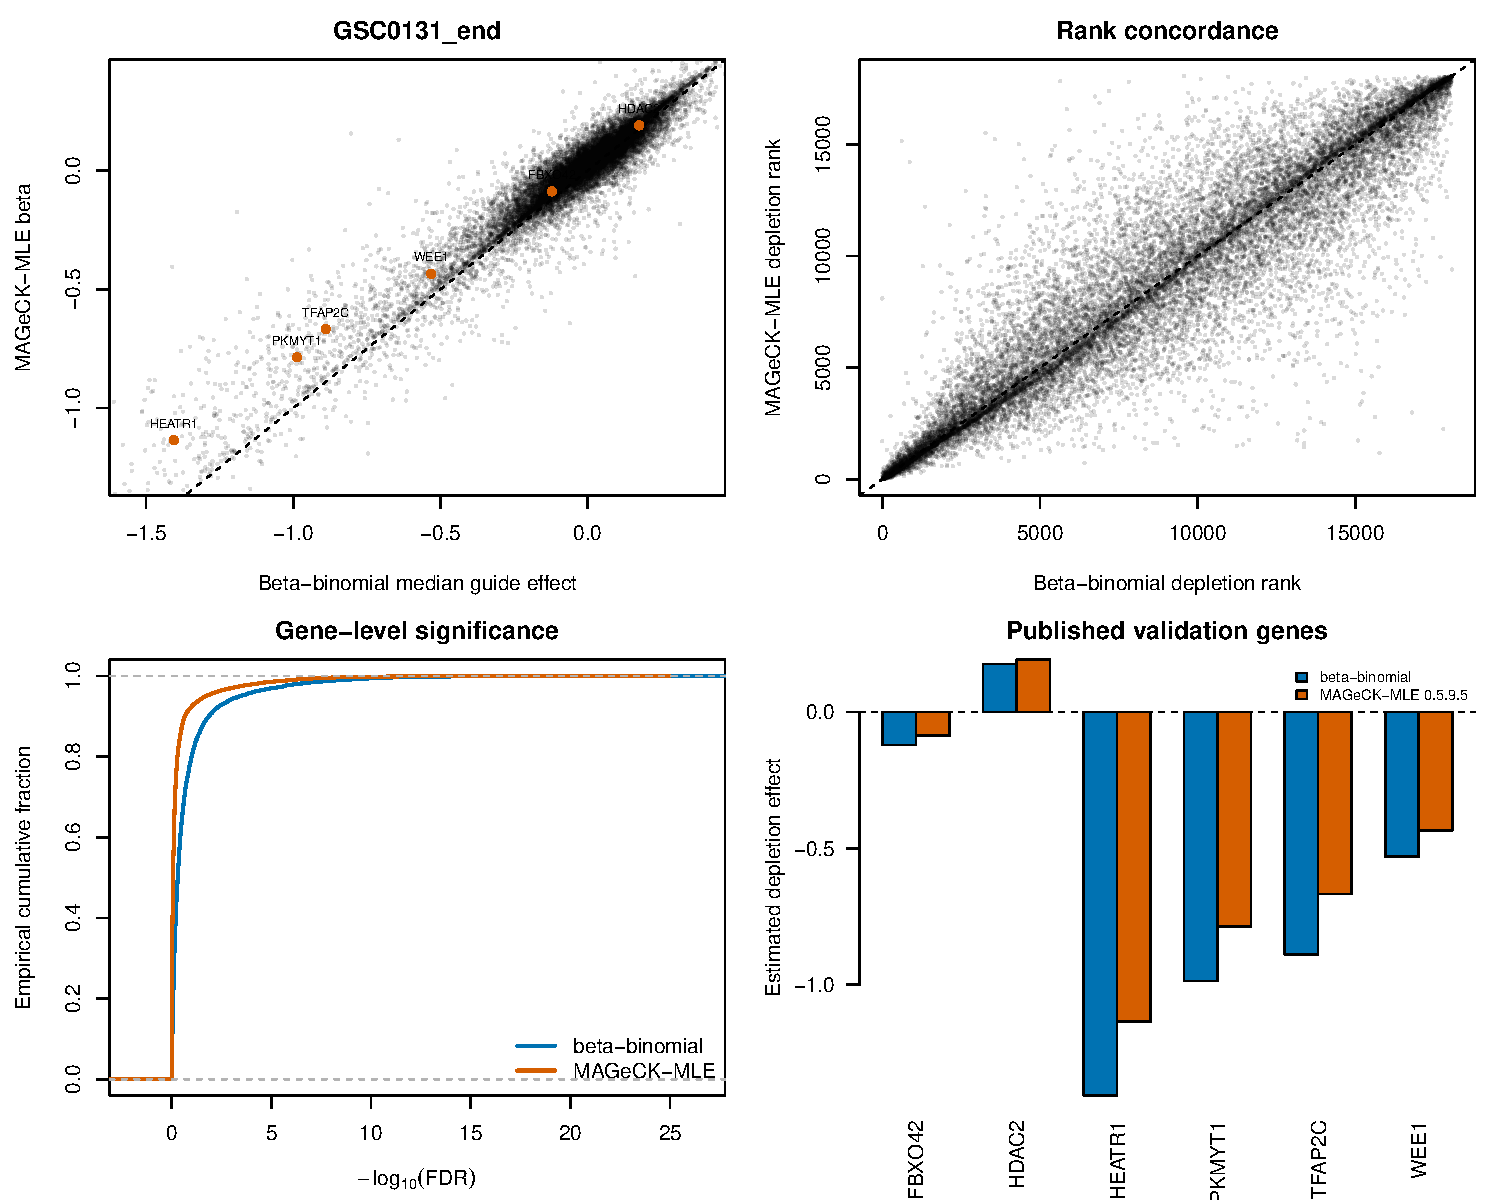
\includegraphics[width=\textwidth]{figures/gse70038_head_to_head.pdf}
\caption{GSE70038 GSC0131 head-to-head.  (A) Gene effects, with dark points
marking the prespecified genes PKMYT1, HEATR1, TFAP2C, FBXO42, HDAC2, and WEE1.
(B) Depletion-rank concordance.  (C) Gene-level FDR distributions.  (D)
Effects for the published validation genes.}
\label{fig:gse}
\end{figure}
\clearpage

% !TeX root = ../../main.tex
\subsection{Endpoint benchmark and copy-number audit}

To ask which method ranks biological dependencies better, we used the
Brunello A375 negative-selection screen of \citet{sanson2018optimized}, bundled
with CB\textsuperscript{2}.  This is an ordinary endpoint screen rather than a
continuous-phenotype experiment, but it supplies an external target unavailable
in GSE70038: reference essential genes should rank ahead of reference
nonessential genes \citep{hart2017evaluation}.  The beta-binomial score combines guide
evidence by directional Stouffer aggregation; the MAGeCK score uses the
official MLE beta and Wald $p$-value.  Both are oriented so larger scores mean
stronger depletion.

\subsubsection{Copy-number-aware analysis}

Copy number is a gene-level property of A375, not a sample-level covariate:
for a given guide it is constant across the plasmid and three terminal
libraries.  Adding it directly to the four-row sample design would therefore
be non-identifiable with the endpoint effect.  Instead, we downloaded the
A375 gene-level profile (ACH-000219) from DepMap Public 19Q3
\citep{depmap19q3,meyers2017cnv} and used MAGeCK 0.5.9.5's official
\texttt{--cnv-norm} piecewise correction.  For an apples-to-apples comparison,
the same MAGeCK piecewise normalizer was applied to the beta-binomial
within-gene median effects.  It adjusts effect sizes after model fitting; it
does not refit either count likelihood.  The common CNV-complete evaluation set
contains 1,506 essential and 869 nonessential genes.

\begin{table}[ht]
\centering
\caption{CNV-aware Sanson A375 benchmark.  The final column is Spearman
correlation between effect and copy number among reference nonessential genes;
values nearer zero indicate less residual CNV-associated depletion.  F1 uses
nominal FDR 0.05 and a negative effect.  Higher discrimination metrics and
CNV correlation closest to zero are highlighted.}
\label{tab:sanson}
\small
\setlength{\tabcolsep}{4pt}
\begin{tabular}{lrrrr}
\toprule
Method & AUROC & Avg. precision & F1 & CNV correlation\\
\midrule
\methodswatch{barcsblue} BARCS &
  \textcolor{barcsblue}{\textbf{0.9598}} & 0.9786 &
  \textcolor{barcsblue}{\textbf{0.8531}} & $-0.185$\\
\methodswatch{barcsblue} BARCS + CNV &
  0.9533 & 0.9762 & \textcolor{barcsblue}{\textbf{0.8531}} & $-0.042$\\
\methodswatch{mageckorange} Official MAGeCK-MLE &
  \textcolor{mageckorange}{\textbf{0.9598}} &
  \textcolor{mageckorange}{\textbf{0.9795}} &
  0.8277 & $-0.207$\\
\methodswatch{mageckorange} Official MAGeCK-MLE + CNV &
  0.9501 & 0.9762 & 0.8277 &
  \textcolor{mageckorange}{$\mathbf{-0.006}$}\\
\bottomrule
\end{tabular}
\end{table}

CNV correction substantially removes the intended nuisance association:
$-0.185$ to $-0.042$ for beta-binomial effects and $-0.207$ to $-0.006$ for
MAGeCK.  It does not improve essential-gene discrimination in this screen.
AUROC decreases by 0.0066 and 0.0097, respectively, and the 0.05-FDR calls are
unchanged.  This is not a contradiction: bias removal and gold-standard
classification are different targets, and amplified genes can include both
dependencies and nondependencies.

After CNV correction, beta-binomial versus MAGeCK global ranking remains
indistinguishable: the AUROC difference is 0.00316 (paired
stratified-bootstrap 95\% CI $-0.00265$ to $0.00924$), and the average
precision difference is effectively zero (95\% CI $-0.00349$ to $0.00295$).
At nominal FDR 0.05, beta-binomial retains 4.18 percentage points more recall
(95\% CI 2.66 to 5.71) and an F1 advantage of 0.0253 (95\% CI 0.0148 to
0.0362).

% !TeX root = ../../main.tex
\subsection{False-discovery conclusions depend on the analysis contract}
\label{sec:fdr-audit}

We audited a deposited Chronos benchmark that compared CB\textsuperscript{2},
MAGeCK, JACKS, DrugZ, and Chronos \citep{dempster2025fdr,
dempster2025fdrdata}.  The key issue was the beta-binomial denominator.  In
the reported null-only Avana analysis, the count matrix was restricted to
control genes before fitting, so its column sums no longer represented full
sequencing depth.  Reusing the full-library CB\textsuperscript{2} probabilities
for the same test genes changed the number of FDR 0.10 discoveries from 152 to
zero.

\begin{table}[htbp]
\centering
\caption{Data-driven audit of the external false-discovery benchmark.
``Known'' refers to the 28 literature-curated condition--gene combinations,
not a complete truth set.}
\label{tab:chronosaudit}
\small
\setlength{\tabcolsep}{4pt}
\begin{tabular}{p{0.18\textwidth}p{0.17\textwidth}p{0.15\textwidth}
                p{0.16\textwidth}p{0.20\textwidth}}
\toprule
Audit & Reference set & Reported result & Full-total reanalysis &
Additional diagnostic\\
\midrule
Avana null-only &
Null genes, five cell lines &
152 calls at FDR 0.10 &
0 calls at FDR 0.10 &
Largest null $p<0.05$ rate: 0.145\\
PSN1 two-versus-two split &
Null pseudo-condition &
0 gene calls &
0 gene calls &
Guide $p<0.05$: 0.0481 raw, 0.0465 scaled\\
DeWeirdt differential screens &
28 curated interactions &
0/28 known recovered &
38 calls; 1/28 known recovered &
37/38 calls arose in one comparison\\
\bottomrule
\end{tabular}
\end{table}

The PSN1 result shows that pooling one guide dispersion across the design can
avoid the extreme loss of power produced by separate two-replicate variance
estimates while retaining a near-nominal guide null.  The DeWeirdt result shows
the boundary of that improvement: BARCS recovered only MCL1 under A-1331852,
and nearly all other calls came from one OVCAR8--olaparib comparison without
recovering BRCA1 or BRCA2.  A global treatment-associated quality shift cannot
be separated from treatment with only two replicates per arm.

These results do not establish a winner against a complete ground truth.
They show that pre-fit guide subsetting and common normalization can alter the
effective depth seen by a library-total-conditional model.  Comparator studies
must preserve full-library totals, separate calibration guides from evaluation
guides, and use blocked permutations or independent validation for
differential screens.

